%-------------------------------------------------------------
% CV en español
% Hugo Ferrando Seage - 2017
%-------------------------------------------------------------

\documentclass[a4paper, 12pt]{article}
\usepackage[utf8]{inputenc}
\usepackage[T1]{fontenc}
\usepackage[spanish]{babel}
\usepackage{subfig}
\usepackage{booktabs}
\usepackage{enumitem} % Customize enumerate items
\usepackage{longtable} % Required to make tables span more than one page
\usepackage{graphicx} % Required for including pictures
\usepackage{multicol}
\usepackage[cm]{fullpage}
\usepackage[usenames,dvipsnames]{xcolor} % Required for specifying custom colors
\usepackage[pdfstartview=Fit]{hyperref} % Required for adding links	and customizing them
\definecolor{linkcolour}{rgb}{0,0.2,0.6} % Link color
\hypersetup{colorlinks,breaklinks,urlcolor=linkcolour,linkcolor=linkcolour, pdfpagemode=UseNone} % Set link colors throughout the document
\hyphenpenalty=10000
\setlength{\columnsep}{-3.5cm}

\begin{document}
\pagestyle{empty} % Removes page numbering

\begin{flushright}
    Graduado en Ingeniería Informática\\
    +34 680 340 463\\
    \href{mailto: me@hugofs.com}{me@hugofs.com}\\
    \href{https://hugofs.com}{hugofs.com}\\
\end{flushright}

\vspace{-27mm} %TODO: Top margin amount

\begin{figure}[ht!]
    \begin{flushleft}
        \subfloat{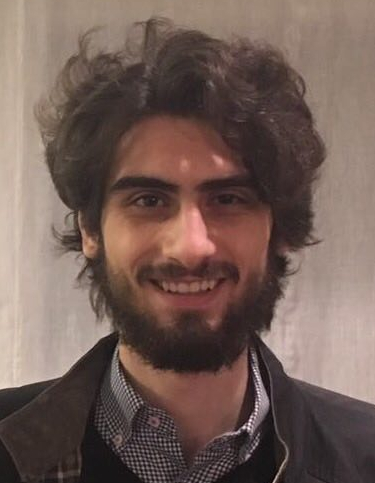
\includegraphics[width=0.13\textwidth]{images/hugo.jpg}}
    \end{flushleft}
\end{figure}

{\textsc {\Huge \vspace{5mm} \hspace{-13mm} Hugo Ferrando Seage}}\\

\begin{longtable}{r|p{12cm}}
    EXPERIENCIA
    & \textbf{Telefónica $\sim$ Talentum Startups/Mood} \hfill sep 16 --
    \\
    & Proyectos en Telefónica I+D \& LUCA
    \\
    & Mejoras del sistema de recomendación content-to-content de Movistar+
    \\\\
    & \textbf{Product Hackers $\sim$ Desarrollador web} \hfill jun 16 -- oct 16
    \\
    & Creación de web apps y chat bots usando Ionic y Angular 2 para móviles y web
    \\\\
    & \textbf{UEM $\sim$ Becas de investigación} \hfill sep 15 -- mar 17
    \\
    & \href{https://www.researchgate.net/publication/314142014_Prediction_of_User_Opinion_for_Products_-_A_Bag-of-Words_and_Collaborative_Filtering_based_Approach}{Modelo de predicción de gustos de usuarios a partir de textos de opinión en Amazon, usando Apache Spark}
    \\
    & Detección de personas en piscinas y playas usando OpenCV para un dron salvavidas
    \\
    & \href{https://github.com/hugo19941994/infrac-coche}{Desarrollo de una app para detectar, alertar y registrar infracciones de tráfico usando OpenCV en Android}
    \\\\
    EDUCACIÓN
    & \textbf{Universidad Europea de Madrid} \hfill 2014 -- 2017
    \\
    & Grado en Ingeniería Informática
    \\
    & \textit{TFG:} \href{https://github.com/hugo19941994/movie-pepper-doc/raw/master/thesis.pdf}{Estudio sobre sistemas de recomendación de películas basados en el procesamiento de lenguaje natural}
    \\
    & \textit{Actividades:} Club de Robotica, Data Science Lab
    \\
    & \textit{Media:} 7.75/10
    \\\\
    & \textbf{Universidad Politécnica de Madrid} \hfill 2012 -- 2014
    \\
    & Grado en Ingeniería Informática
    \\
    & \textit{Actividades:} Capítulo de Estudiantes ACM
    \\\\
    CONOCIMIENTOS
    & \textbf{Lenguajes de Programación}
    \\
    TÉCNICOS
    & Python, C/C++, Java, Javascript (ES6), Bash
    \\\\
    & \textbf{Frameworks}
    \\
    & Apache Spark, React, Angular 4, NLTK, Gensim, Android SDK \& NDK
    \\\\
    & \textbf{Administración de sistemas \& documentación}
    \\
    & GNU/Linux, Git, SSH, GPG, \LaTeX, Markdown, Nginx, Jenkins, OpenVPN, Knot, Postfix, Dovecot
    \\\pagebreak
    PROYECTOS
    & \href{https://github.com/hugo19941994/space-invaders-emu}{Space Invaders emulator}: Ejecuta Space Invaders en Windows
    \\
    & \href{https://github.com/hugo19941994/chip8-emu}{CHIP8 emulator}: Ejecuta programas de CHIP-8 en Windows y Linux
    \\
    & \href{https://vpn.hugofs.com}{ovpn}: Proveedor de VPN basadas en OpenVPN
    \\
    & \href{https://github.com/hugo19941994/ViajeFacil}{ViajeFácil}: Software de gestión para agencias de vuelos. Colaboración entre UEM \& Unisys
    \\
    & \href{https://github.com/hugo19941994/cv-parser}{CV Parser}: Sistema para gestionar CV usando reconocimiento de entidades nombradas y redes bayesianas. Colaboración entre UEM \& Everis
    \\
    & \href{https://github.com/hugo19941994/robot}{Human Rescue Bot}: Ganador del Laureate Awards for Excellence in Robotics Engineering 2016
    \\\\
    CERTIFICACIONES
    & Certificate in Advanced English (CAE)
    \\
    & CCNA 1: Introduction to Networks
    \\
    & CCNA 2: Routing and Switching Essentials
    \\
    & CCNA 4: Connecting Networks
    \\\\
    IDIOMAS
    & \vspace{-1.85\baselineskip} % TODO: Find a better wayy
    \begin{multicols}{2}
        \begin{itemize}[leftmargin=0cm, label={}, noitemsep]
            \item Español nativo
            \item Inglés avanzado
            \item Italiano nativo
            \item Francés básico
        \end{itemize}
    \end{multicols}
\end{longtable}
\end{document}
